\chapter{Oxidación y reducción de los alquenos}\label{ch:b2:alkene-redox}

El pegamento epoxi de dos componentes viene en dos tubos: uno contiene moléculas que terminan en
anillos \omterm{def:b2:alkene-redox:epoxide}{epóxido}, anillos de tres eslabones con dos carbonos y un oxígeno; el otro, una
amina. Al mezclarlos, los anillos tensionados se abren uno tras otro y la pasta fragua
formando una red dura. Los alquenos son la materia prima de esos anillos, de alcoholes
situados donde la regla de Markovnikov nunca los pondría, de dioles con una geometría
elegida y de los pequeños fragmentos que en otro tiempo indicaban a los químicos dónde estaba un doble
enlace en una molécula. Este capítulo añade a las adiciones electrófilas del
volumen del primer año las reacciones que reducen u oxidan el doble enlace, y
la estereoquímica que impone cada una.

\begin{recall}
El volumen del primer año: adiciones electrófilas, regla de Markovnikov, iones halonio,
adiciones sin y anti, hidratación de los alquenos, niveles de oxidación del carbono,
dadores de hidruro, quimioselectividad, compuestos meso y mezclas racémicas,
reacciones estereoespecíficas. \Cref{ch:b2:catalytic-cycles}: el ciclo de hidrogenación del
catalizador de Wilkinson.
\end{recall}

\begin{omfigure}
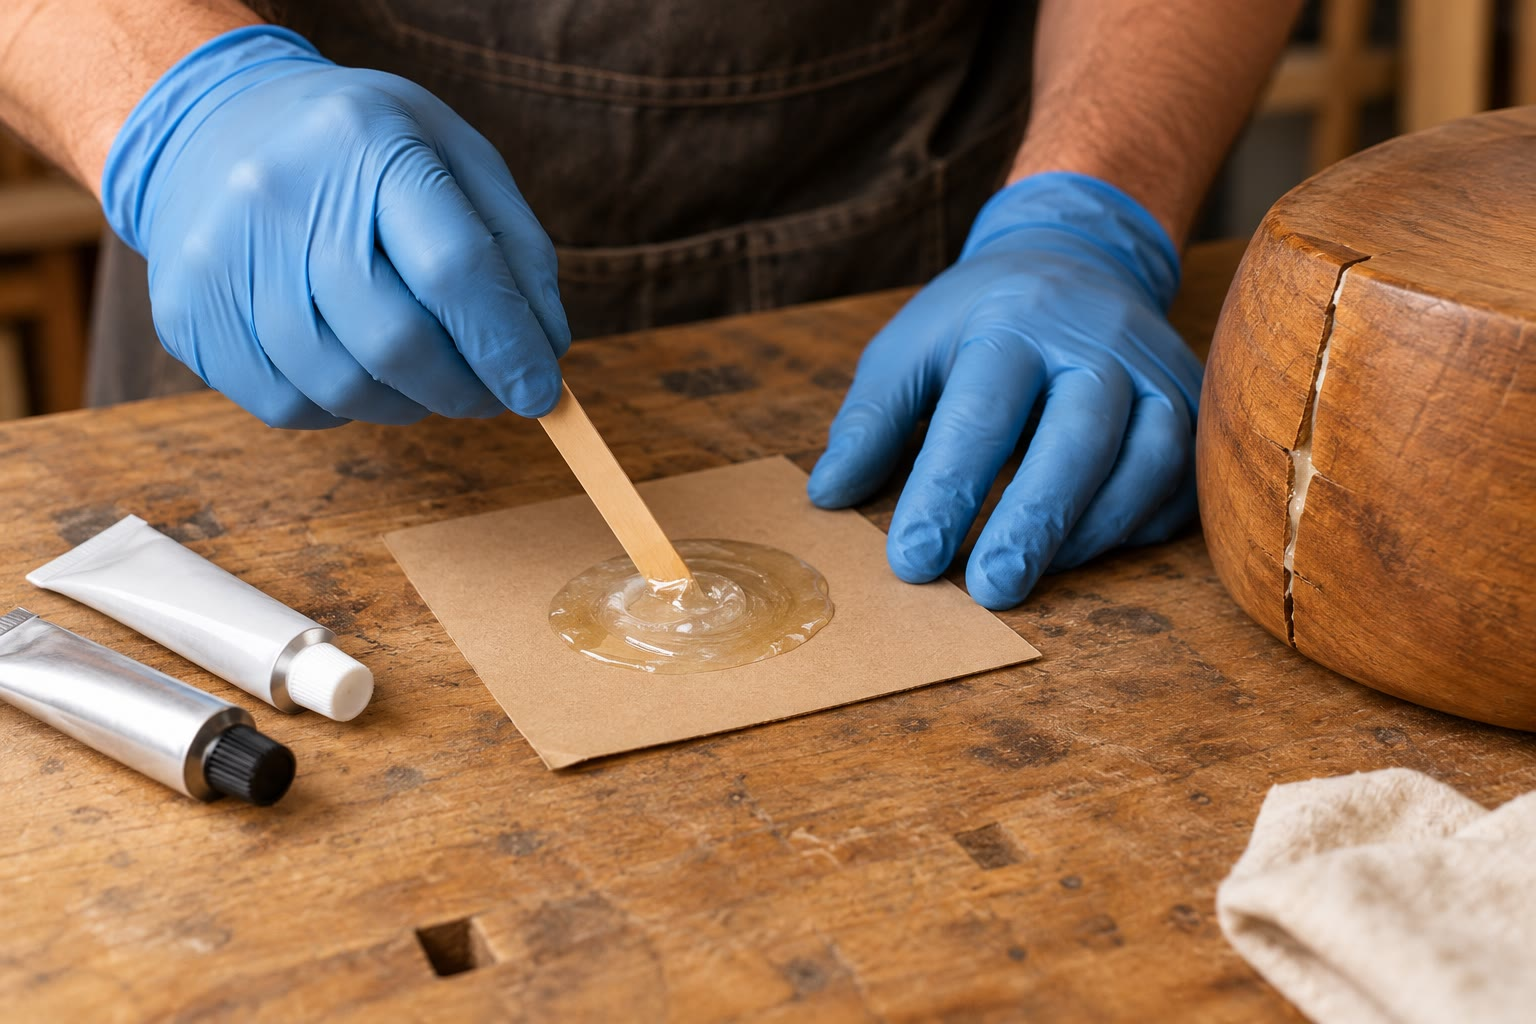
\includegraphics[width=0.6\linewidth]{images/book3/ai/b2-21-epoxy.jpg}

{\small Mezcla de un pegamento epoxi de dos componentes: la resina, con grupos \omterm{def:b2:alkene-redox:epoxide}{epóxido}, y el
endurecedor, una amina, reaccionan en cuanto se encuentran; los anillos se abren y unen las moléculas
en una red sólida.}
\end{omfigure}

\section{Hidrogenación catalítica}

\begin{definition}[Hidrogenación catalítica]\label{def:b2:alkene-redox:hydrogenation}
Una \emph{hidrogenación catalítica}\index{hidrogenacion catalitica@hidrogenación catalítica} adiciona dihidrógeno a un
enlace múltiple en presencia de un catalizador: un metal finamente dividido (paladio sobre
carbono, platino, níquel) en catálisis heterogénea, o un complejo soluble como el
de Wilkinson en catálisis homogénea.
\end{definition}

Sobre una superficie metálica quedan retenidos tanto el dihidrógeno como el alqueno, el enlace \ce{H-H} se rompe
dando átomos de hidrógeno superficiales, y estos se transfieren uno tras otro a los átomos de carbono
del alqueno, que yace plano sobre el metal.

\begin{proposition}[Adición sin]\label{prop:b2:alkene-redox:syn-hydrogenation}
La \omterm{def:b2:alkene-redox:hydrogenation}{hidrogenación catalítica} aporta los dos átomos de hidrógeno por la misma cara del doble enlace.
Un alquino hidrogenado sobre un catalizador de paladio envenenado se detiene en el alqueno, que es el
isómero (\textit{Z}).
\end{proposition}

\begin{proof}[Argumento]
El alqueno está unido al catalizador por una cara, y ambos hidrógenos proceden del
catalizador, por esa cara: adición sin. Con un alquino, los dos hidrógenos añadidos al
triple enlace quedan del mismo lado, en cis entre sí: el (\textit{Z})-alqueno. Un catalizador
parcialmente desactivado (paladio sobre carbonato de calcio con una sal de plomo y quinoleína)
retiene el alquino mucho más fuertemente que el alqueno formado, que abandona la superficie
antes de una segunda adición.
\end{proof}

\section{Hidroboración--oxidación}

\begin{definition}[Hidroboración]\label{def:b2:alkene-redox:hydroboration}
Una \emph{hidroboración}\index{hidroboracion@hidroboración} adiciona un enlace B--H de un borano a un
enlace \ce{C=C}; seguida de una oxidación con peróxido de hidrógeno alcalino, convierte el
alqueno en un alcohol cuyo grupo hidroxilo está sobre el carbono menos sustituido: una
\emph{orientación anti-Markovnikov}\index{orientacion anti-Markovnikov@orientación anti-Markovnikov}.
\end{definition}

\begin{omfigure}
\setchemfig{atom sep=1.8em}
\schemestart[][west]
\chemfig{H_3C-[:30]CH=[:-30]CH_2}
\+ \chemfig{H-BH_2}
\arrow{->[adición sin]}
\chemfig{H_3C-[:30]CH_2-[:-30]CH_2-[:30]BH_2}
\arrow{->[\ce{H2O2}][\ce{HO-}]}
\chemfig{H_3C-[:30]CH_2-[:-30]CH_2-[:30]OH}
\schemestop
\par\vspace{6pt}

{\small Hidroboración--oxidación del propeno. El borano se adiciona en una sola etapa, el boro al
carbono terminal y el hidrógeno al interno, ambos por la misma cara; la oxidación
sustituye el boro por \ce{OH} con retención de configuración. Se forma propan-1-ol, no el
propan-2-ol de la hidratación catalizada por ácido.}
\end{omfigure}

\begin{proposition}[Orientación de la hidroboración]\label{prop:b2:alkene-redox:hydroboration-regio}
El boro se adiciona al carbono menos sustituido del doble enlace, y el hidrógeno al más
sustituido; la adición es sin.
\end{proposition}

\begin{proof}[Argumento]
El boro, con un orbital p vacío, es el electrófilo: en el estado de transición de cuatro centros
(los dos carbonos, el boro y el hidrógeno), el enlace con el boro se forma un poco antes que el enlace C--H, y una
carga parcial positiva aparece sobre el otro carbono, mejor estabilizada por el más
sustituido; el voluminoso grupo borado prefiere además el extremo menos impedido. Ambos enlaces nuevos
se forman por una misma cara, en una etapa concertada: sin.
\end{proof}

\begin{proposition}[Oxidación con retención]\label{prop:b2:alkene-redox:retention}
La oxidación de un alquilborano por peróxido de hidrógeno alcalino sustituye cada enlace C--B por un
enlace C--OH con retención de configuración en el carbono.
\end{proposition}

\begin{proof}[Argumento]
El anión hidroperóxido se adiciona al boro; un grupo alquilo migra entonces del boro al
oxígeno contiguo, con su par de electrones, mientras sale el hidróxido; el carbono conserva sus enlaces
del mismo lado durante todo el proceso. La hidrólisis del enlace B--O libera el alcohol.
\end{proof}

\section{Epóxidos}

\begin{definition}[Epóxido]\label{def:b2:alkene-redox:epoxide}
Un \emph{epóxido}\index{epoxido@epóxido} (oxirano) es un éter cíclico con un anillo de tres eslabones de
dos carbonos y un oxígeno. Una \emph{epoxidación}\index{epoxidacion@epoxidación} convierte un alqueno en
un epóxido, normalmente con un \emph{peroxiácido}\index{peroxiacido@peroxiácido} \ce{RCO3H}, que transfiere
un átomo de oxígeno al doble enlace.
\end{definition}

\begin{omfigure}
\setchemfig{atom sep=2em}
\schemestart
\chemfig{R-[:30]CH=[:-30]CH-[:30]R}
\+ \chemfig{Ar-C(=[2]O)-O-O-H}
\arrow{->}
\chemfig{[:-60]CH(-[:210]R)*3(-CH(-[:-30]R)-O-)}
\+ \chemfig{Ar-C(=[2]O)-OH}
\schemestop
\par\vspace{6pt}

{\small \omterm{def:b2:alkene-redox:epoxide}{Epoxidación} por un \omterm{def:b2:alkene-redox:epoxide}{peroxiácido} (Ar: por ejemplo, un grupo 3-clorofenilo). El oxígeno
terminal del \omterm{def:b2:alkene-redox:epoxide}{peroxiácido} se transfiere al doble enlace en una sola etapa, y ambos enlaces C--O
se forman por la misma cara.}
\end{omfigure}

\begin{proposition}[Epoxidación estereoespecífica]\label{prop:b2:alkene-redox:epoxidation}
La \omterm{def:b2:alkene-redox:epoxide}{epoxidación} por un \omterm{def:b2:alkene-redox:epoxide}{peroxiácido} es estereoespecífica: un (\textit{Z})-alqueno da el \omterm{def:b2:alkene-redox:epoxide}{epóxido} cis,
y un (\textit{E})-alqueno, el \omterm{def:b2:alkene-redox:epoxide}{epóxido} trans.
\end{proposition}

\begin{proof}
El oxígeno se transfiere en una sola etapa concertada a una cara del doble enlace, que no
gira entretanto: las posiciones relativas de los sustituyentes se conservan.
\end{proof}

\begin{proposition}[Apertura de los epóxidos]\label{prop:b2:alkene-redox:opening}
Un nucleófilo abre un \omterm{def:b2:alkene-redox:epoxide}{epóxido} atacando un carbono por la cara opuesta al oxígeno
(apertura anti, con inversión en ese carbono). En condiciones básicas ataca el carbono menos
impedido; en condiciones ácidas, el más sustituido.
\end{proposition}

\begin{proof}[Argumento]
La tensión del anillo hace fáciles de romper los enlaces C--O. Con un nucleófilo fuerte y sin ácido,
la apertura es una sustitución bimolecular, y el carbono menos impedido es el que se alcanza con más
facilidad. En medio ácido el oxígeno se protona; el enlace C--O con el carbono más sustituido
es el que más se alarga, pues ese carbono lleva la mayor carga parcial positiva, e incluso un nucleófilo
débil (agua, un alcohol) ataca allí, de nuevo por detrás y, por tanto, en anti.
\end{proof}

\begin{omfigure}
\setchemfig{atom sep=2em}
\schemestart
\chemfig{[:-60]C(-[:210]H_3C)(-[:150]H_3C)*3(-CH_2-O-)}
\arrow{->[\ce{CH3O-}][\ce{CH3OH}]}[,1.4]
\chemfig{H_3C-C(-[2]CH_3)(-[6]OH)-CH_2-OCH_3}
\schemestop

\medskip
\schemestart
\chemfig{[:-60]C(-[:210]H_3C)(-[:150]H_3C)*3(-CH_2-O-)}
\arrow{->[\ce{CH3OH}][\ce{H+}]}[,1.4]
\chemfig{H_3C-C(-[2]CH_3)(-[6]OCH_3)-CH_2-OH}
\schemestop
\par\vspace{6pt}

{\small Apertura del 2,2-dimetiloxirano por el metanol. Arriba, con metóxido: ataque en el
\ce{CH2}, el carbono menos impedido. Abajo, en medio ácido: ataque en el carbono más sustituido,
que soporta la mayor parte de la carga positiva del \omterm{def:b2:alkene-redox:epoxide}{epóxido} protonado.}
\end{omfigure}

\section{Dihidroxilación}

\begin{definition}[Dihidroxilación]\label{def:b2:alkene-redox:dihydroxylation}
Una \emph{dihidroxilación}\index{dihidroxilacion@dihidroxilación} convierte un alqueno en un 1,2-diol añadiendo
un grupo \ce{OH} a cada carbono del doble enlace.
\end{definition}

El tetróxido de osmio, en cantidad catalítica con un reoxidante, y el permanganato diluido en frío añaden
los dos oxígenos a través de un éster cíclico, por una cara: una \omterm{def:b2:alkene-redox:dihydroxylation}{dihidroxilación} sin. La \omterm{def:b2:alkene-redox:epoxide}{epoxidación}
seguida de apertura con agua en medio ácido da el diol anti.

\begin{proposition}[Dioles sin y anti]\label{prop:b2:alkene-redox:diols}
A partir del (\textit{Z})-but-2-eno, la \omterm{def:b2:alkene-redox:dihydroxylation}{dihidroxilación} sin da el meso-butano-2,3-diol, y la vía del \omterm{def:b2:alkene-redox:epoxide}{epóxido}
da los dioles (2\textit{R},3\textit{R}) y (2\textit{S},3\textit{S}) en mezcla racémica; a partir del
(\textit{E})-but-2-eno, los resultados se intercambian.
\end{proposition}

\begin{proof}
En el (\textit{Z})-but-2-eno los dos metilos están del mismo lado. Añadir dos \ce{OH} por una cara
da un diol en el que, escrito en la conformación eclipsada del antiguo doble enlace, los
dos \ce{OH} están de un lado y los dos metilos del otro: un plano de simetría pasa entre
C2 y C3; es el compuesto meso. La vía del \omterm{def:b2:alkene-redox:epoxide}{epóxido} pone los dos \ce{OH} en caras opuestas
(anti): el plano de simetría se pierde, y el ataque a uno u otro carbono del \omterm{def:b2:alkene-redox:epoxide}{epóxido} aquiral,
igualmente probable, da los dos enantiómeros en cantidades iguales. Para el (\textit{E})-alqueno, cada
etapa cambia la relación entre los metilos, lo que intercambia los resultados.
\end{proof}

\begin{omfigure}
\begin{tikzpicture}[font=\small]
  \begin{scope}
    \draw[thick] (0,0) -- (0,1.2);
    \draw[thick] (0,1.2) -- (-0.7,1.45); \draw[thick] (0,1.2) -- (0.7,1.45);
    \node[anchor=east] at (-0.7,1.45) {\ce{HO}}; \node[anchor=west] at (0.7,1.45) {\ce{CH3}};
    \draw[thick] (0,0) -- (-0.7,0.25); \draw[thick] (0,0) -- (0.7,0.25);
    \node[anchor=east] at (-0.7,0.25) {\ce{HO}}; \node[anchor=west] at (0.7,0.25) {\ce{CH3}};
    \node[anchor=south] at (0,1.25) {\scriptsize H};
    \node[anchor=north] at (0,-0.05) {\scriptsize H};
    \draw[densely dashed, omThm] (-1.6,0.6) -- (1.6,0.6);
    \node at (0,-1.0) {sin: meso};
  \end{scope}
  \begin{scope}[xshift=6.5cm]
    \draw[thick] (0,0) -- (0,1.2);
    \draw[thick] (0,1.2) -- (-0.7,1.45); \draw[thick] (0,1.2) -- (0.7,1.45);
    \node[anchor=east] at (-0.7,1.45) {\ce{HO}}; \node[anchor=west] at (0.7,1.45) {\ce{CH3}};
    \draw[thick] (0,0) -- (-0.7,0.25); \draw[thick] (0,0) -- (0.7,0.25);
    \node[anchor=east] at (-0.7,0.25) {\ce{H3C}}; \node[anchor=west] at (0.7,0.25) {\ce{OH}};
    \node[anchor=south] at (0,1.25) {\scriptsize H};
    \node[anchor=north] at (0,-0.05) {\scriptsize H};
    \node[align=center] at (0,-1.1) {anti: un enantiómero\\ (formado con su imagen especular)};
  \end{scope}
\end{tikzpicture}

{\small Los dos butano-2,3-dioles a partir del (\textit{Z})-but-2-eno, esquema (enlace C2--C3
vertical, con los dos grupos de cada carbono dibujados a izquierda y derecha). La adición sin pone los dos
\ce{OH} del mismo lado: un plano de simetría interno (discontinuo), el compuesto meso. La adición anti
los pone en lados opuestos: un diol quiral, formado junto con su enantiómero.}
\end{omfigure}

\section{Ruptura oxidante}

\begin{definition}[Ruptura oxidante]\label{def:b2:alkene-redox:cleavage}
Una \emph{ruptura oxidante}\index{ruptura oxidante} rompe los dos enlaces de un doble enlace \ce{C=C}
y convierte cada carbono en un grupo carbonilo o carboxilo. En una
\emph{ozonólisis}\index{ozonolisis@ozonólisis}, el alqueno reacciona con el ozono y el ozónido
intermedio se descompone en una segunda etapa, el tratamiento.
\end{definition}

\begin{proposition}[Productos de la ozonólisis]\label{prop:b2:alkene-redox:ozonolysis}
La \omterm{def:b2:alkene-redox:cleavage}{ozonólisis} divide cada enlace \ce{C=C} en dos grupos \ce{C=O}. Con un tratamiento reductor
(cinc y ácido, o sulfuro de dimetilo), un carbono que lleva un hidrógeno da un aldehído; con
un tratamiento oxidante (peróxido de hidrógeno), da un ácido carboxílico. Un carbono que lleva dos
grupos carbonados da una cetona en ambos casos.
\end{proposition}

\begin{proof}[Argumento]
El ozono se adiciona al doble enlace, el intermedio se reorganiza y el enlace C--C se rompe, dando
un ozónido en el que cada antiguo carbono alquénico está unido a dos oxígenos. El tratamiento lo reduce
a dos compuestos carbonílicos, o bien oxida además los aldehídos. Las etapas intermedias se
admiten.
\end{proof}

\begin{omfigure}
\setchemfig{atom sep=2em}
\schemestart
\chemfig{H_3C-[:30]C(-[:90]CH_3)=[:-30]CH-[:30]CH_3}
\arrow{->[1. \ce{O3}][2. \ce{Zn}, \ce{H+}]}[,1.8]
\chemfig{H_3C-C(=[2]O)-CH_3}
\+
\chemfig{H-C(=[2]O)-CH_3}
\schemestop
\par\vspace{6pt}

{\small \omterm{def:b2:alkene-redox:cleavage}{Ozonólisis} del 2-metilbut-2-eno con un tratamiento reductor: propanona y
etanal. Volver a unir los dos carbonos carbonílicos mediante un doble enlace reconstruye el
alqueno.}
\end{omfigure}

\begin{method}[Localizar un doble enlace]\label{met:b2:alkene-redox:locate-double-bond}
\begin{enumerate}
  \item Enumérense los fragmentos carbonílicos de la \omterm{def:b2:alkene-redox:cleavage}{ozonólisis} y cuéntense sus carbonos; deben sumar
        los del alqueno.
  \item Cada carbono de \ce{C=O} era un carbono doblemente enlazado: únanse los fragmentos sustituyendo dos
        \ce{C=O} por un \ce{C=C}.
  \item Para un anillo, sale una sola molécula con dos grupos carbonilo; únanse sus dos extremos.
  \item Compruébese con la fórmula y el grado de insaturación.
\end{enumerate}
\end{method}

El permanganato concentrado en caliente también rompe los dobles enlaces, dando ácidos y cetonas; el
peryodato de sodio rompe los 1,2-dioles en dos compuestos carbonílicos, una vía más suave a través del diol.

\begin{method}[Elegir un reactivo para un alqueno]\label{met:b2:alkene-redox:choose-reagent}
\begin{center}
\small
\renewcommand{\arraystretch}{1.15}
\begin{tabular}{lll}
objetivo & reactivo & estereoquímica, orientación \\ \hline
alcano & \ce{H2}, Pd/C & sin \\
alcohol de Markovnikov & \ce{H2O}, ácido & vía un carbocatión \\
alcohol anti-Markovnikov & \ce{BH3}, luego \ce{H2O2}, \ce{HO-} & sin \\
\omterm{def:b2:alkene-redox:epoxide}{epóxido} & \omterm{def:b2:alkene-redox:epoxide}{peroxiácido} & estereoespecífica \\
diol sin & \ce{OsO4} (cat.) o \ce{MnO4-} en frío & sin \\
diol anti & \omterm{def:b2:alkene-redox:epoxide}{peroxiácido}, luego \ce{H2O}, ácido & anti \\
dos carbonilos & \ce{O3}, luego \ce{Zn}/ácido & ruptura \\
\end{tabular}
\end{center}
\end{method}

\begin{safety}{\ghs[5mm]{GHS02}\,\ghs[5mm]{GHS03}\,\ghs[5mm]{GHS05}\,\ghs[5mm]{GHS06}}
El tetróxido de osmio es volátil y muy tóxico (daña los ojos); se usa en cantidad catalítica
en disolución, en una vitrina de gases. Los \omterm{def:b2:alkene-redox:epoxide}{peroxiácidos} y el peróxido de hidrógeno son oxidantes que
pueden descomponerse violentamente si se calientan o se concentran; las disoluciones de borano son inflamables;
el ozono es tóxico y se genera en una vitrina.
% ledger: ghs:OsO4, ghs:mCPBA, ghs:BH3-THF, ghs:O3, ghs:NaIO4
\end{safety}

\section{Ejercicios}

\begin{exercise}[$\star$]\label{exo:b2:alkene-redox:1}
Dese el producto del 1-metilciclohexeno con: \ce{H2}/Pd; \ce{H2O}/\ce{H+};
\ce{BH3} y luego \ce{H2O2}/\ce{HO-}; un \omterm{def:b2:alkene-redox:epoxide}{peroxiácido}; \ce{OsO4} (cat.); \ce{O3} y luego
\ce{Zn}/\ce{H+}.
\end{exercise}

\begin{exercise}[$\star$]\label{exo:b2:alkene-redox:2}
¿Qué alcohol da la hidroboración--oxidación del 2-metilpropeno? ¿Y la hidratación catalizada
por ácido?
\end{exercise}

\begin{exercise}[$\star$]\label{exo:b2:alkene-redox:3}
Dibújese el \omterm{def:b2:alkene-redox:epoxide}{epóxido} formado a partir del (\textit{E})-but-2-eno. ¿Es quiral?
\end{exercise}

\begin{exercise}[$\star$]\label{exo:b2:alkene-redox:4}
Dense los productos de la \omterm{def:b2:alkene-redox:cleavage}{ozonólisis} del hex-3-eno con un tratamiento reductor y luego con un
tratamiento oxidante.
\end{exercise}

\begin{exercise}[$\star\star$]\label{exo:b2:alkene-redox:5}
Dense los dioles formados a partir del (\textit{Z})-but-2-eno (a) con \ce{OsO4}; (b) con un \omterm{def:b2:alkene-redox:epoxide}{peroxiácido}
y luego ácido acuoso. ¿Cuál es ópticamente inactivo por ser meso, y cuál
por ser racémico?
\end{exercise}

\begin{exercise}[$\star\star$]\label{exo:b2:alkene-redox:6}
El 2,2-dimetiloxirano se abre con agua en medio ácido y con hidróxido. ¿Dan las dos vías el
mismo producto? Explíquese.
\end{exercise}

\begin{exercise}[$\star\star$]\label{exo:b2:alkene-redox:7}
¿Cómo se prepararía el (\textit{Z})-hex-3-eno a partir del hex-3-ino?
\end{exercise}

\begin{exercise}[$\star\star$]\label{exo:b2:alkene-redox:8}
Un alqueno \ce{C7H14} da, por \omterm{def:b2:alkene-redox:cleavage}{ozonólisis} con un tratamiento reductor, propanona y butanal.
Dese su estructura.
\end{exercise}

\begin{exercise}[$\star\star$]\label{exo:b2:alkene-redox:9}
Propóngase una síntesis del hexan-1-ol a partir del hex-1-eno, y dígase por qué la hidratación catalizada
por ácido fracasaría.
\end{exercise}

\begin{exercise}[$\star\star\star$]\label{exo:b2:alkene-redox:10}
El limoneno tiene un doble enlace trisustituido en el anillo y uno exocíclico disustituido
(\ce{C(CH3)=CH2}). ¿Cuál reacciona primero con un equivalente de un \omterm{def:b2:alkene-redox:epoxide}{peroxiácido}, y cuál con
un equivalente de un borano voluminoso? Explíquese.
\end{exercise}

\begin{exercise}[$\star\star\star$]\label{exo:b2:alkene-redox:11}
Prepárense el trans-ciclohexano-1,2-diol a partir del ciclohexeno y el cis-ciclohexano-1,2-diol.
\end{exercise}

\begin{exercise}[$\star\star\star$]\label{exo:b2:alkene-redox:12}
Un compuesto \ce{C6H10} absorbe un equivalente de \ce{H2}. Su \omterm{def:b2:alkene-redox:cleavage}{ozonólisis} con un tratamiento
reductor da un único producto, el hexanodial \ce{OHC-(CH2)4-CHO}. Identifíquese.
\end{exercise}

\section{Problema: identificar un terpeno}

\begin{problem}[{Problema de fin de semana --- la fórmula y la insaturación del limoneno, su
hidrogenación, los fragmentos de su ozonólisis y las reacciones selectivas de sus dos
dobles enlaces}]
\label{pb:b2:alkene-redox:1}
El limoneno, el aroma de la piel de naranja, tiene la fórmula \ce{C10H16}. Es el
1-metil-4-(prop-1-en-2-il)ciclohex-1-eno: un doble enlace en el anillo que lleva un metilo, y un
grupo exocíclico \ce{C(CH3)=CH2} en el carbono opuesto del anillo. $R =
\qty{8.314}{J/(K.mol)}$; masas molares (\unit{g/mol}): C 12.011, H 1.008.
% ledger: aw:C, aw:H, const:R, ghs:limonene

\medskip
\noindent\textbf{Parte I --- Fórmula e hidrogenación.}
\begin{enumerate}
  \item Calcúlese la masa molar del limoneno.
  \item Calcúlese su grado de insaturación.
  \item ¿Cuántos anillos y cuántos dobles enlaces tiene?
  \item Escríbase su hidrogenación sobre paladio, producto incluido.
  \item Calcúlese la cantidad de dihidrógeno absorbida por \qty{1.00}{g} de limoneno.
  \item Calcúlese su volumen a \qty{25}{\degreeCelsius} y \qty{1.00}{bar}.
  \item ¿Es quiral el producto?
\end{enumerate}

\medskip
\noindent\textbf{Parte II --- \omterm{def:b2:alkene-redox:cleavage}{Ozonólisis}.}
\begin{enumerate}[resume]
  \item ¿Qué fragmentos da la \omterm{def:b2:alkene-redox:cleavage}{ozonólisis} con un tratamiento reductor? (Cuéntense los carbonos.)
  \item ¿Por qué el doble enlace del anillo da una molécula y no dos?
  \item ¿Qué fragmento se pierde como gas o como líquido volátil?
  \item ¿En qué se diferenciarían los productos con un tratamiento oxidante?
  \item Muéstrese cómo los fragmentos localizan los dos dobles enlaces.
  \item ¿Cuántos estereocentros tiene el limoneno, y lo conserva la \omterm{def:b2:alkene-redox:cleavage}{ozonólisis}?
\end{enumerate}

\medskip
\noindent\textbf{Parte III --- \omterm{def:b2:alkene-redox:hydroboration}{Hidroboración}.}
\begin{enumerate}[resume]
  \item Con un equivalente de un borano voluminoso, ¿qué doble enlace reacciona? ¿Por qué?
  \item Dibújese el producto tras la oxidación.
  \item ¿Es el nuevo alcohol primario, secundario o terciario?
  \item ¿Por qué se llama anti-Markovnikov esta orientación?
  \item ¿Cuántos estereoisómeros pueden formarse en el nuevo estereocentro?
  \item ¿Qué reactivo pondría en cambio el \ce{OH} sobre el carbono más sustituido del
        mismo doble enlace?
\end{enumerate}

\medskip
\noindent\textbf{Parte IV --- \omterm{def:b2:alkene-redox:epoxide}{Epoxidación}.}
\begin{enumerate}[resume]
  \item Con un equivalente de un \omterm{def:b2:alkene-redox:epoxide}{peroxiácido}, ¿qué doble enlace reacciona? ¿Por qué?
  \item Dibújese el \omterm{def:b2:alkene-redox:epoxide}{epóxido}.
  \item Ábrase con agua en medio ácido: ¿en qué carbono ataca el agua?
  \item Dibújese el diol y dese la orientación relativa de sus dos \ce{OH}.
  \item ¿Cómo se obtendría el otro diastereoisómero de este diol?
  \item Indíquese el volumen de dihidrógeno absorbido por \qty{1.00}{g} de limoneno a
        \qty{25}{\degreeCelsius} y \qty{1}{bar}.
\end{enumerate}
\end{problem}
